% !TEX root = SegwayDoku.tex
\renewcommand{\autoren}{Timo Veit}
\newpage
\section{Auslegung Kurvengeschwindigkeit}

\begin{figure}[h]  % [h] bedeutet, dass das Bild genau an dieser Stelle im Text erscheint
\centering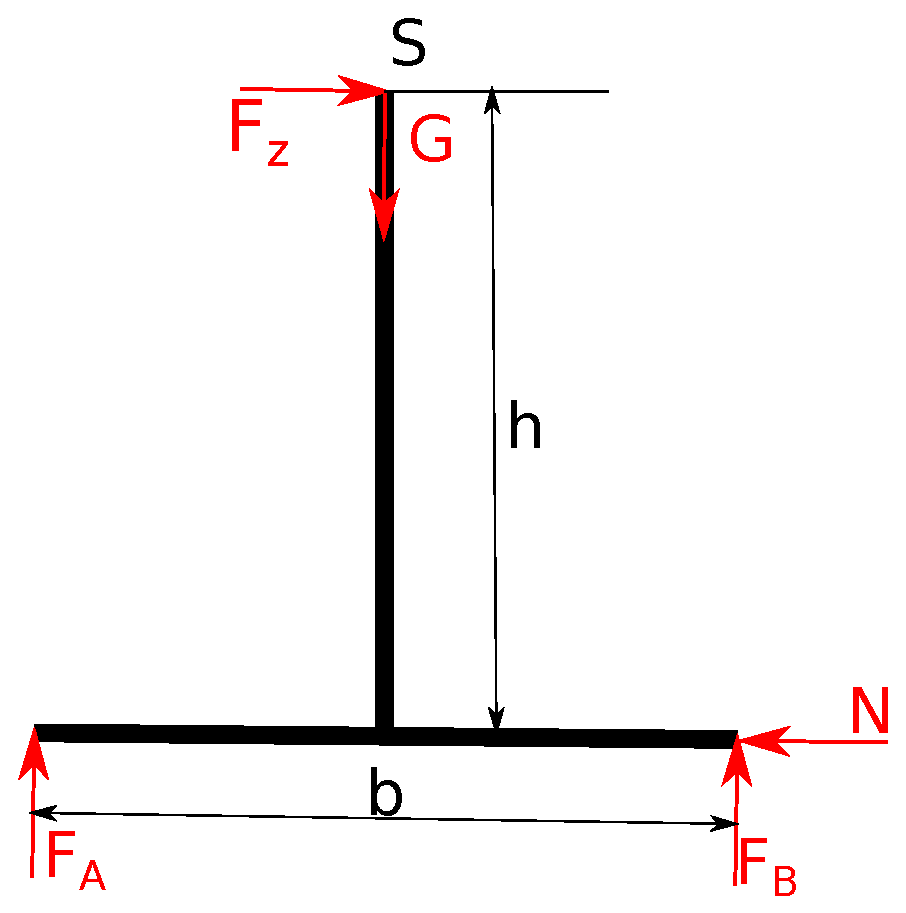
\includegraphics[width=0.6\textwidth]{images/SegwayFliehkraft.eps}
\caption{Kräfte bei der Kurvenfahrt \newline (Quelle: eigene Darstellung)}
\label{zentripetal}
\end{figure}

Bei der Kurvenfahrt darf der Roboter nicht seitlich umkippen. Um dies zu gewährleisten, muss das Verhältnis zwischen Geschwindigkeit und Kurvenradius passen. Dazu soll der innere Reifen noch mindestens die Hälfte der Last aufnehmen wie im Stand also ein Viertel der Gewichtskraft.

Es gilt:
\begin{flalign}
    % durch das & Zeichen werden alle Gleichungen an diesem Punkt ausgerichtet
	F_A &  = \frac{1}{4} m \cdot g
	\label{eq:gewichtskraft_1} \\
	G &  = m \cdot g
	\label{eq:gewichtskraft_2} \\
	F_{z} & = m \cdot \ddot x
	\label{eq:zentrifugalkraft} \\
	N & = m \cdot \frac{v^{2}}{r}
	\label{eq:zentripetalkraft} \\
	F_{A} + F_{B} & = G
	\label{eq:vertikale} \\
	N & = F_{z}
	\label{eq:horizontale} \\
    F_A \cdot b & = F_z \cdot h
	\label{eq:moment}
\end{flalign}

Hieraus folgt:
% hier keine Leerzeile machen, sonst wird der Abstand ganz groß
\begin{flalign}
    \ddot x & = \frac{v^{2}}{r}
	\label{eq:xpp} \\
    \frac{1}{4} m \cdot g \cdot b & = m \cdot \frac{v^{2}}{r} \cdot h
	\label{eq:lsg_1} 
\end{flalign}

Und daraus die Zusammenhänge von Geschwindigkeit zu Radius
\begin{flalign}
    v & = \sqrt{\dfrac{gb}{4h} \cdot r}
	\label{eq:lsg_v} \\
    r & = \dfrac{4h}{gb} \cdot v^2
	\label{eq:lsg_r} 
\end{flalign}

Der notwendige Reibwert \(\mu\) zwischen Reifen und Boden ergibt sich aus der Haftbedingung.

\begin{flalign}
    \mu \cdot mg & = m \cdot \frac{v^{2}}{r}
	\label{eq:mu_1} \\
    \mu & = \frac{v^{2}}{rg}
	\label{eq:mu_2} 
\end{flalign}